% !TEX TS-program = XeLaTeX
\documentclass[tikz,dvipsnames]{standalone}
\usepackage{pgfgantt}
\usepackage{fontspec}
% Main font
\setmainfont{LinLibertine_R.otf}[%
  Ligatures=TeX,%
  BoldFont=LinLibertine_RB.otf,%
  ItalicFont=LinLibertine_RI.otf,%
  BoldItalicFont=LinLibertine_RBI.otf]
% Sans font
\setsansfont{LinBiolinum_R.ttf}[%
    Ligatures=TeX,%
    BoldFont=LinBiolinum_RB.ttf,%
    ItalicFont=LinBiolinum_RI.ttf]
\begin{document}
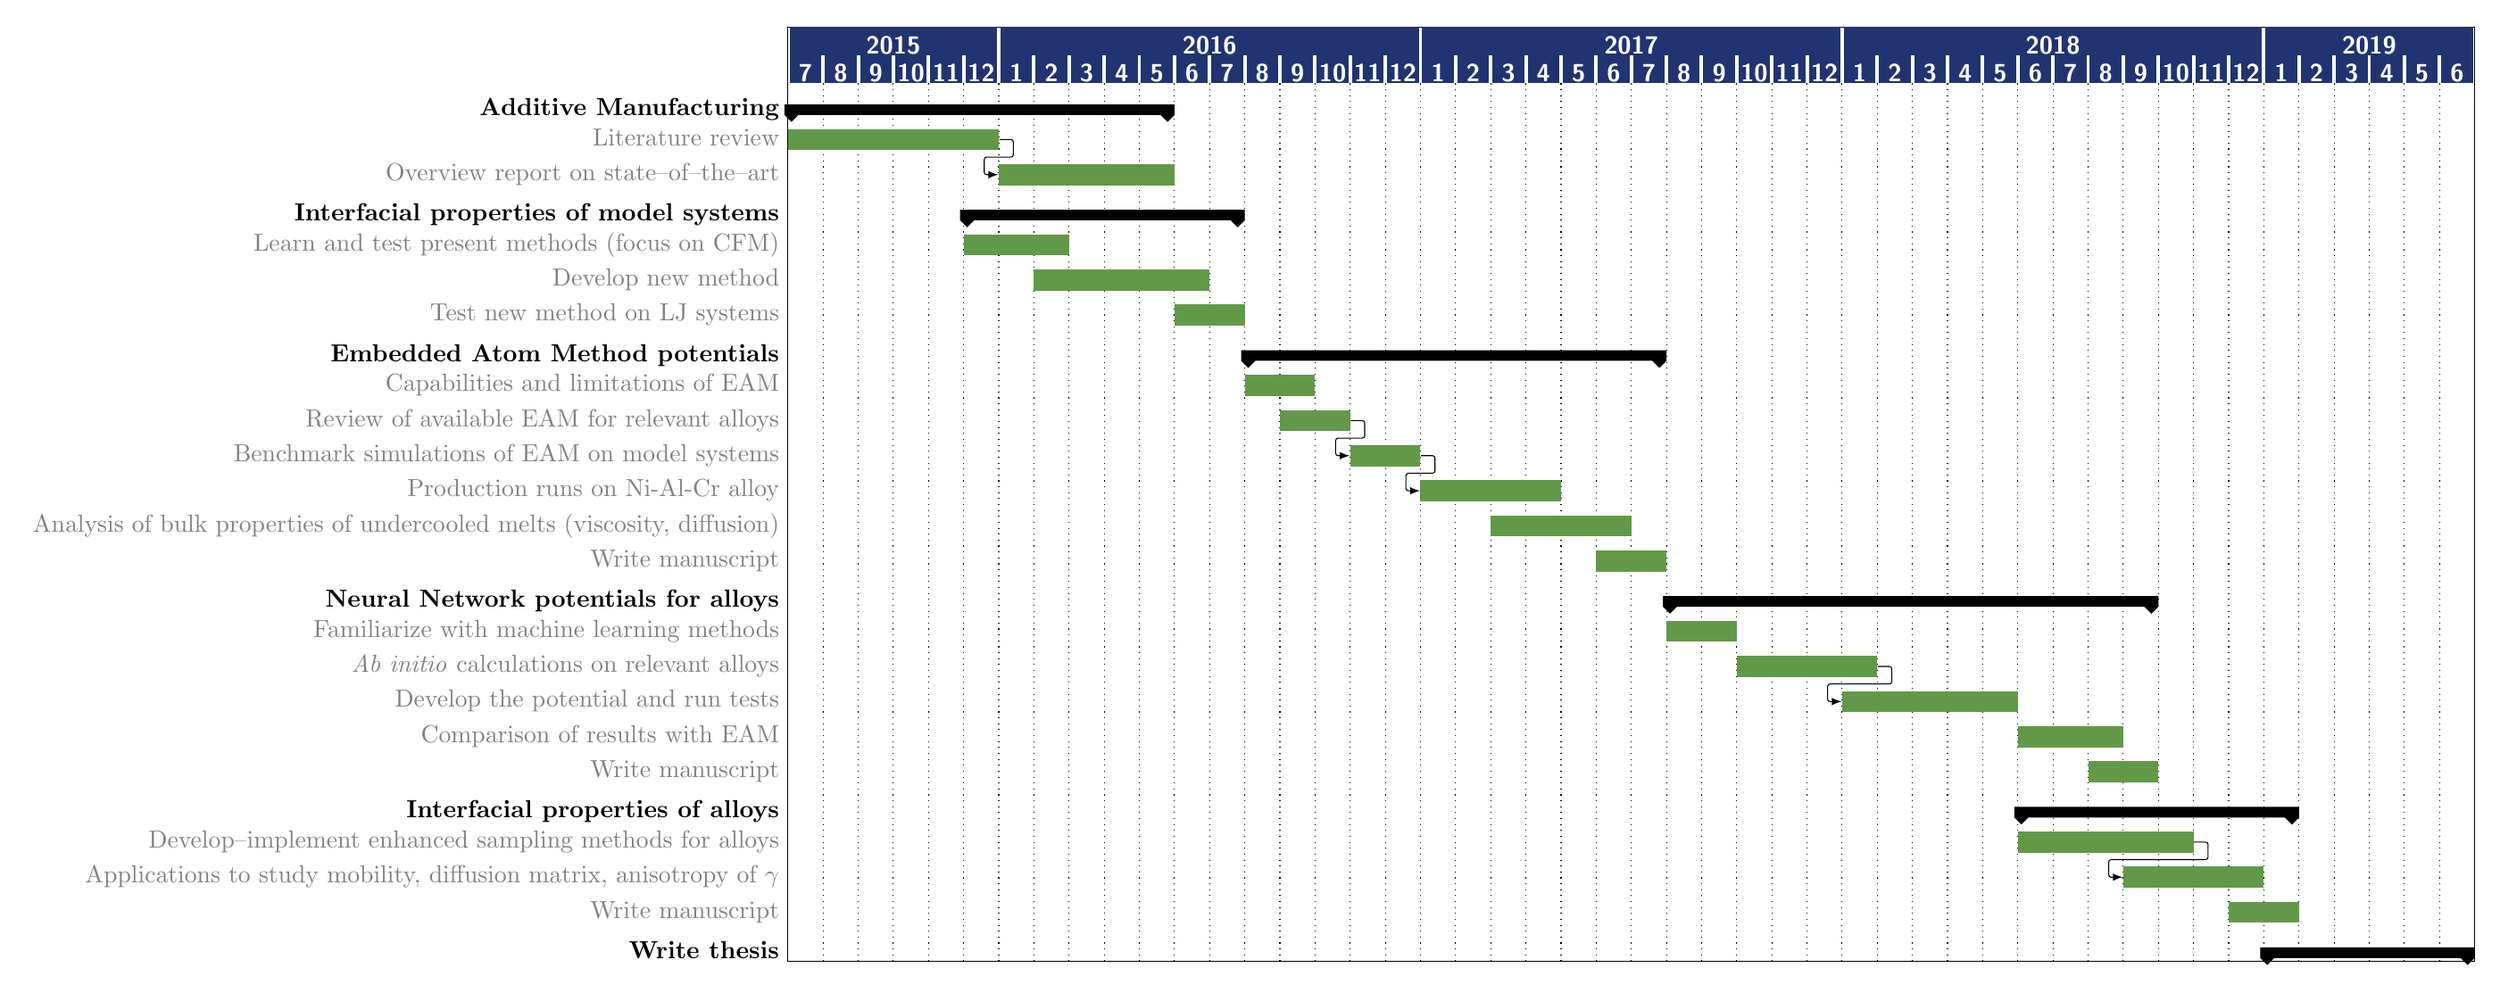
\begin{tikzpicture}
\begin{ganttchart}[
        y unit title=0.4cm,
        y unit chart=0.5cm,
        vgrid,
        time slot format=simple,
        %compress calendar,
        title/.append style={draw=none, fill=RoyalBlue!50!black},
        title label font=\sffamily\bfseries\color{white},
        title label node/.append style={below=-1.6ex},
        title left shift=.05,
        title right shift=-.05,
        title height=1,
        bar/.append style={draw=none, fill=OliveGreen!75},
        bar height=.6,
        bar label font=\normalsize\color{black!50},
        group right shift=0,
        group top shift=.6,
        group height=.3,
        group peaks height=.2,
        bar incomplete/.append style={fill=Maroon}
        ]{1}{48}
    \gantttitle{2015}{6}
    \gantttitle{2016}{12}
    \gantttitle{2017}{12}
    \gantttitle{2018}{12}
    \gantttitle{2019}{6} \\
    %
    \gantttitlelist{7,...,12}{1}
    \gantttitlelist{1,...,12}{1}
    \gantttitlelist{1,...,12}{1}
    \gantttitlelist{1,...,12}{1}
    \gantttitlelist{1,...,6}{1} \\
    %
    \ganttgroup{Additive Manufacturing}{1}{11} \\
    \ganttbar{Literature review}{1}{6} \\
    \ganttlinkedbar{Overview report on state--of--the--art}{7}{11}
    \ganttnewline
    %
    \ganttgroup{Interfacial properties of model systems}{6}{13}\\
    \ganttbar{Learn and test present methods (focus on CFM)}{6}{8}\\
    \ganttbar{Develop new method}{8}{12}\\
    \ganttbar{Test new method on LJ systems}{12}{13}
    \ganttnewline
    %
    \ganttgroup{Embedded Atom Method potentials}{14}{25}\\
    \ganttbar{Capabilities and limitations of EAM}{14}{15}\\
    \ganttbar{Review of available EAM for relevant alloys}{15}{16}\\
    \ganttlinkedbar{Benchmark simulations of EAM on model systems}{17}{18}\\
    \ganttlinkedbar{Production runs on Ni-Al-Cr alloy}{19}{22}\\
    \ganttbar{Analysis of bulk properties of undercooled melts (viscosity, diffusion)}{21}{24}\\
    \ganttbar{Write manuscript}{24}{25}
    \ganttnewline
    %
    \ganttgroup{Neural Network potentials for alloys}{26}{39}\\
    \ganttbar{Familiarize with machine learning methods}{26}{27}\\
    \ganttbar{\textit{Ab initio} calculations on relevant alloys}{28}{31}\\
    \ganttlinkedbar{Develop the potential and run tests}{31}{35}\\
    \ganttbar{Comparison of results with EAM}{36}{38}\\
    \ganttbar{Write manuscript}{38}{39}\ganttnewline
    %
    \ganttgroup{Interfacial properties of alloys}{36}{43}\\
    \ganttbar{Develop--implement enhanced sampling methods for alloys}{36}{40}\\
    \ganttlinkedbar{Applications to study mobility, diffusion matrix, anisotropy of $\gamma$}{39}{42}\\
    \ganttbar{Write manuscript}{42}{43}\ganttnewline
    %
    \ganttgroup{Write thesis}{43}{48}
    %%%%
    %\ganttmilestone{Milestone}{7} \ganttnewline
    %\ganttbar{Final Task}{8}{12}
    %\ganttlink{elem2}{elem3}
    %\ganttlink{elem3}{elem4}
\end{ganttchart}
\end{tikzpicture}
\end{document}





